\section{Evaluation}
\label{sec:evaluation}

\subsection{Determining the Optimized DEW-Acc Setup}
\label{subsec:dew_acc_width}
The DEWA window is already fixed at $(T_{\mathrm{drop}}, T_{\mathrm{replace}})=(9,3)$.
The remaining hardware parameter is the bit-width of the integer accumulator.
A wider DEW-Acc overflows less often and therefore issues fewer FP-Acc requests on the normal path, but the adder, shifter, and register all grow with the width.

We sweep 12--32 bits on LLaMA2-7B under W-BFP4 / T2A-BiE4 (G16), using one frozen activation stream so that the width is the only variable.
FP-Acc activity here is the overflow-event count; outlier requests do not depend on the width and are left out of this curve.
PE area is the synthesized area of the full PE at each width.

\begin{figure}[t]
    \centering
    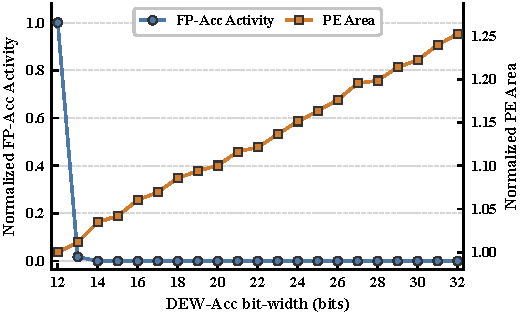
\includegraphics[width=\linewidth]{figures/dew_acc_activity_area_tradeoff.pdf}
    \caption{Normalized FP-Acc overflow activity and synthesized PE area versus DEW-Acc bit-width on LLaMA2-7B (W-BFP4 / T2A-BiE4, G16, $(T_{\mathrm{drop}}, T_{\mathrm{replace}})=(9,3)$). Both series are normalized to W12.}
    \label{fig:dew_acc_width}
\end{figure}

Fig.~\ref{fig:dew_acc_width} shows both series normalized to W12.
W13 is the better choice: overflow activity drops sharply while PE area barely grows, so we use a 13-bit DEW accumulator.

\subsection{Hardware and Energy Comparison}
\label{subsec:hw_energy}
We compare three synthesized PEs in TSMC 90\,nm at 100\,MHz: a conventional BFP4 baseline, a Bucket Getter PE~\cite{bucketgetter2023}, and the proposed PE with the 13-bit DEW accumulator of Section~\ref{subsec:dew_acc_width}.
Fig.~\ref{fig:pe_area_energy} reports cell area and energy, each normalized to the baseline.

\begin{figure}[h]
    \centering
    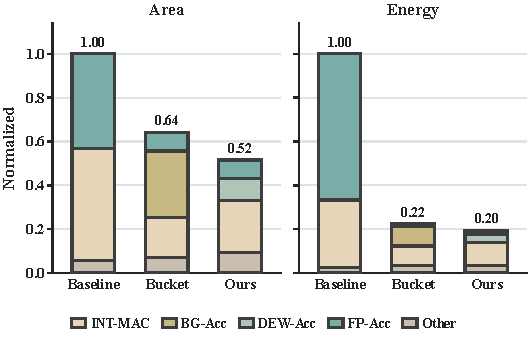
\includegraphics[width=\linewidth]{figures/pe_area_energy_comparison.pdf}
    \caption{Normalized PE area and energy of a BFP4 baseline, a Bucket Getter PE, and the proposed PE (TSMC 90\,nm, 100\,MHz). Both metrics are normalized to the baseline.}
    \label{fig:pe_area_energy}
\end{figure}

The proposed PE is smaller than both the baseline and Bucket Getter.
Its energy is close to that of Bucket Getter and well below the baseline.
